%%%------------------------------------------------------------------------------------%%
%%%------------------------------------------------------------------------------------%%
%%% Content: Open-Science-Poster LaTeX Scaffold 
%%% Usage: Collaborative scientific poster writing 
%%% Author: Claas-Thido Pfaff
%%%------------------------------------------------------------------------------------%%
%%%------------------------------------------------------------------------------------%%

%%%------------------------------------------------------------------------------%%%
%%% Document class: open_science_poster (Based on beamer and beamer poster) %%%
%%%------------------------------------------------------------------------------%%%
%%
%

\documentclass[gray]{subdocuments/open_science_poster}\usepackage{graphicx, color}
%% maxwidth is the original width if it is less than linewidth
%% otherwise use linewidth (to make sure the graphics do not exceed the margin)
\makeatletter
\def\maxwidth{ %
  \ifdim\Gin@nat@width>\linewidth
    \linewidth
  \else
    \Gin@nat@width
  \fi
}
\makeatother

\IfFileExists{upquote.sty}{\usepackage{upquote}}{}
\definecolor{fgcolor}{rgb}{0.2, 0.2, 0.2}
\newcommand{\hlnumber}[1]{\textcolor[rgb]{0,0,0}{#1}}%
\newcommand{\hlfunctioncall}[1]{\textcolor[rgb]{0.501960784313725,0,0.329411764705882}{\textbf{#1}}}%
\newcommand{\hlstring}[1]{\textcolor[rgb]{0.6,0.6,1}{#1}}%
\newcommand{\hlkeyword}[1]{\textcolor[rgb]{0,0,0}{\textbf{#1}}}%
\newcommand{\hlargument}[1]{\textcolor[rgb]{0.690196078431373,0.250980392156863,0.0196078431372549}{#1}}%
\newcommand{\hlcomment}[1]{\textcolor[rgb]{0.180392156862745,0.6,0.341176470588235}{#1}}%
\newcommand{\hlroxygencomment}[1]{\textcolor[rgb]{0.43921568627451,0.47843137254902,0.701960784313725}{#1}}%
\newcommand{\hlformalargs}[1]{\textcolor[rgb]{0.690196078431373,0.250980392156863,0.0196078431372549}{#1}}%
\newcommand{\hleqformalargs}[1]{\textcolor[rgb]{0.690196078431373,0.250980392156863,0.0196078431372549}{#1}}%
\newcommand{\hlassignement}[1]{\textcolor[rgb]{0,0,0}{\textbf{#1}}}%
\newcommand{\hlpackage}[1]{\textcolor[rgb]{0.588235294117647,0.709803921568627,0.145098039215686}{#1}}%
\newcommand{\hlslot}[1]{\textit{#1}}%
\newcommand{\hlsymbol}[1]{\textcolor[rgb]{0,0,0}{#1}}%
\newcommand{\hlprompt}[1]{\textcolor[rgb]{0.2,0.2,0.2}{#1}}%

\usepackage{framed}
\makeatletter
\newenvironment{kframe}{%
 \def\at@end@of@kframe{}%
 \ifinner\ifhmode%
  \def\at@end@of@kframe{\end{minipage}}%
  \begin{minipage}{\columnwidth}%
 \fi\fi%
 \def\FrameCommand##1{\hskip\@totalleftmargin \hskip-\fboxsep
 \colorbox{shadecolor}{##1}\hskip-\fboxsep
     % There is no \\@totalrightmargin, so:
     \hskip-\linewidth \hskip-\@totalleftmargin \hskip\columnwidth}%
 \MakeFramed {\advance\hsize-\width
   \@totalleftmargin\z@ \linewidth\hsize
   \@setminipage}}%
 {\par\unskip\endMakeFramed%
 \at@end@of@kframe}
\makeatother

\definecolor{shadecolor}{rgb}{.97, .97, .97}
\definecolor{messagecolor}{rgb}{0, 0, 0}
\definecolor{warningcolor}{rgb}{1, 0, 1}
\definecolor{errorcolor}{rgb}{1, 0, 0}
\newenvironment{knitrout}{}{} % an empty environment to be redefined in TeX

\usepackage{alltt}

% Class options:
% 	colors: gray, blue, green, red, orange (default = grey) 
% 	head separator: default on (switch off with: noheadsep)
%  long, wide (switch between orientation)

%%%------------------------------------------------------------------------------%%%
%%% Load user options %%%
%%%------------------------------------------------------------------------------%%%

%%%------------------------------------------------------------------------------------%%
%%%------------------------------------------------------------------------------------%%
%%% Content : Open-Science-Poster LateX-Style 
%%% Use : Open-Sciene-Poster user modifications 
%%% Author : Claas-Thido Pfaff
%%%------------------------------------------------------------------------------------%%
%%%------------------------------------------------------------------------------------%%

%%%-------------------------------------------------%%%
%%% Define own colors %%%
%%%-------------------------------------------------%%%

% Example:
%  \xdefinecolor{YourColor}{rgb}{0,0,0.4}

%%%-------------------------------------------------%%%
%%% Set the poster title %%%
%%%-------------------------------------------------%%%

\title{Open-Science-Poster Title}
\author{Author One \and Author Two}
\institute{Affiliation here}
\date{\today}

%%%-------------------------------------------------%%%
%%% Define own commands %%%
%%%-------------------------------------------------%%%

% Example:
%  \newcommand{name}[number of parameters]{things to do}

%%%-------------------------------------------------%%%
%%% Define own environments %%%
%%%-------------------------------------------------%%%

% Example:
%  \newenvironment{name}[number of parameters]{definition begin}{definition end}

%%%-------------------------------------------------%%%
%%% Set PDF options %%%
%%%-------------------------------------------------%%%

% Example:
%  \hypersetup{%
%   pdfauthor={Your-Name},
%   pdfcreator={Your-Name},
%   pdfsubject={Subject},
%   pdfkeywords={Keyword1, Keyword2, ...}
%  }
% 

%%%-------------------------------------------------%%%
%%% Additional bib options %%%
%%%-------------------------------------------------%%%

% \ExecuteBibliographyOptions{
% url=false,
% isbn=false,
% doi=false,
% firstinits=false,
% bibencoding=utf8
% }

%% add a BibTeX bibliography file %%
% \addbibresource{subdocuments/open_science_paper.bib}
 

%%%------------------------------------------------------------------------------%%%
%%% Begin the document %%%
%%%------------------------------------------------------------------------------%%%

\begin{document}

%%%--------------------------------------------------------------%%%
%%% Document preparations %%%
%%%--------------------------------------------------------------%%%
%%
%

%%%-------------------------------------------------%%%
%%% Preferences for Knitr %%%
%%%-------------------------------------------------%%%


%%%-------------------------------------------------%%%
%%% Sub document global preferences for Knitr %%%
%%%-------------------------------------------------%%%








%%%--------------------------------------------------------------%%%
%%% Document content %%%
%%%--------------------------------------------------------------%%%
%%
%

\begin{frame}[t]
	\begin{columns}[t] 
		%% First column %%%
		\begin{column}{0.28\paperwidth} 

			\begin{alertblock}{Abstract}
				\lipsum[1]
			\end{alertblock}

			\begin{alertblock}{Questions}
				\begin{itemize}
					\item One?
					\item Two?
					\item Three?
				\end{itemize}
			\end{alertblock}

			\begin{block}{Introduction}
				\lipsum[1-2]	
			\end{block}

			\begin{exampleblock}{}
				\begin{figure}[H] % {{{
				% Label fig:test_plot
				\centering
				\begin{tikzpicture}
					\node[pictureframe]{%    
						\begin{minipage}{0.95\textwidth}%
							\begin{center}
\begin{knitrout}
\definecolor{shadecolor}{rgb}{0.969, 0.969, 0.969}\color{fgcolor}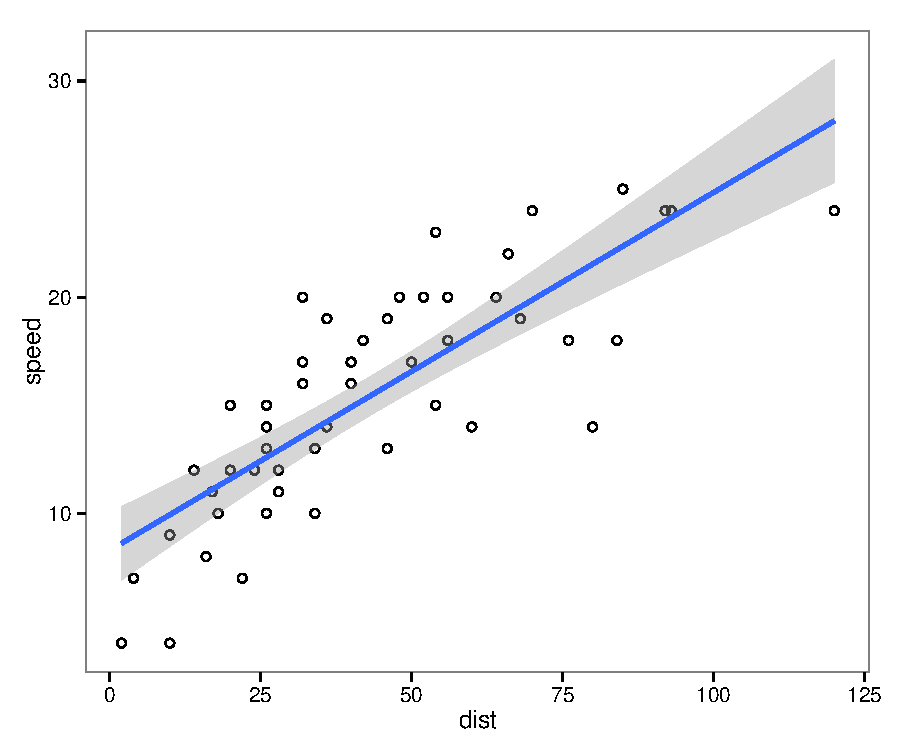
\includegraphics[width=\textwidth]{graphics/dynamic/test_plot} 
\end{knitrout}

							\end{center}
						\end{minipage}
					};
				\end{tikzpicture}
				\caption{Lorem ipsum dolor sit amet, consectetuer adipiscing elit. Aenean
				commodo ligula eget dolor. Aenean massa. Cum sociis natoque penatibus et
				magnis dis parturient montes, nascetur ridiculus mus. Donec quam felis,
				ultricies nec, pellentesque eu, pretium quis, sem.}
				\label{fig:test_plot}
			\end{figure} % }}}
		\end{exampleblock}

%% End first column %%%
		\end{column}


	%% Second column %%%
	\begin{column}{0.28\paperwidth}

			\begin{block}{Material and Methods}
				\lipsum[2]


			\end{block}

		%% End second column %%%
		\end{column}


		%% Third column %%%
		\begin{column}{0.28\paperwidth}

			\begin{alertblock}{Answers}
				\begin{itemize}
					\item One!
					\item Two!
					\item Three!
				\end{itemize}
			\end{alertblock}

			\begin{exampleblock}{}
				\lipsum[2-3]	
			\end{exampleblock}

		\end{column}  


	\end{columns}
\end{frame}

\end{document}
